%------------------------------------------------
\section{Méthodes de calculs existantes}
%------------------------------------------------

%-----------------------------------------------------------------
\subsection{Suivi de Bord}
%-----------------------------------------------------------------

La méthode du suivi du bord d'un bord d'un disque discret est un processus étudié et connu. Elle est sensiblement la même suivant le cas souhaité : 4-connexes ou 8-connexes. Elle se décompose en deux étapes. Trouver un point sur le bord, puis chercher les points suivants jusqu'à retrouver le premier point.
% on - nous

%-----------------------------------------------------------------
\subsubsection{Trouver le sommet de départ}

Pour lancer l'algorithme, il faut rechercher un point sur le bord du disque. Nous avons choisi de récupérer le point d'ordonnée minimale et d'abscisse maximal à l'intérieur du disque. Par concstruction, ce point appartient toujours au bord. Pour ce faire, nous prenons le point de $\mathcal{Z}^2$ possédant les coordonnées entières de notre centre. À partir de ce point, nous descendons le long de l'axe verticale d'une longueur entière égale au rayon pour trouver un point d'ordonnée miniamle. Ensuite, nous tranlatons suivant l'axe horizontal afin de trouver le point d'abscisse maximal. On note a notre point de départ. 

\begin{figure}[h!]
  \centering
  \includegraphics[width=0.4\linewidth,page=1]{fig/4-exi/suivi/exi-depart-0.pdf}
  \includegraphics[width=0.4\linewidth,page=1]{fig/4-exi/suivi/exi-depart-1.pdf}
  \caption{Suivi de bord 4-connexes et 8-connexes}
\end{figure}
  

%-----------------------------------------------------------------
\subsubsection{Trouver le sommet suivant}

La deuxième étape consiste à trouver le sommet suivant de appartenant à notre bord et d'itérer cette étape tant que le bord du disque n'est pas refermé.

Le sommet suivant est choisi suivant la position des 4-voisins (resp 8-voisins) et du sens de rotation. Pour notre étude nous avons délibérément pris le parti de tourner dans le sens trigonométrique. En partance de notre point de départ et afin de tourner dans le sens trigonométrique nous choisirons le premier voisin à l'intérieur parmi le choix ordonnée de $\left\{E, N, O, S\right\}$ dans le cas 4-connnexes(resp :  $\left\{E, NE, N, NO, O, SO, S, SE \right\}$ dans le cas 8-connexes).

\begin{figure}[h!]
  \centering
  \includegraphics[width=0.4\linewidth,page=1]{fig/4-exi/suivi/exi-suivi-0.pdf}
  \caption{Suivi de bord 4-connexes et 8-connexes}
\end{figure}
  

%-----------------------------------------------------------------
\subsection{Enveloppe Convexe : Algorithme de Har-Peled}
%-----------------------------------------------------------------

Le calcul de l'enveloppe convexe est particulièrement étudié. De nombreux algorithmes existes : Parcours de Graham, Marche de Jarvis... 

Une méthode particulièrement performante à néanmoins retenue notre attention. Elle a été introduite par Har-Peled en 98 \cite{HarPeled98}. Il y présente un algorithme de calcul de l'enveloppe convexe qui est incrémental et output sensitive.


\begin{Definition}{Output sensitive}\\
\label{def:os}
      Un algorithme output sensitive possède un temps d’exécution qui dépend de la taille de la sortie.
\end{Definition}

Dans ce cas de figure bien précis, la méthode présentée dépend du nombre de sommets de notre enveloppe convexe. \\

La méthode permet de construire successivement et rapidement les arêtes de notre polygone. Elle s'appuie sur le calcul de convergents, qui représente le pendant géométrique du calcul du pgcd de deux nombres entiers. 
En effet, il a été démontré dans ce même article que la complexité en temps de cette algorithme de calcul de l'enveloppe convexe d'un disque de rayon $R_D$ révèle d'une part de la recherche du prochain sommet en $O(log R_D)$ et également du nombre de sommet qui est $O( R_{D}^{2/3})$. Soit une complexité totale en temps de  $O( R_{D}^{2/3} log R_D)$.


%-----------------------------------------------------------------
\subsubsection{Calcul des convergents}

Cette méthode de calcul est géométrique. On transforme notre deux nombres entiers $x, y$ en un point de $\mathbb{Z}^{2}$ qu'on appellera $P = (P_x, P_y)$. À partir de l’origine $O=(0,0)$, on va chercher à trouver le premier point appartenant au segment de droite [O,P]. Le coefficient trouvé correspondant finalement au pgcd de $P_x$ et $P_y$.\\

Pour cela on met en place une méthode récursive.\\
Soient $p_{-2} = (1,0)$ et $p_{-1} = (0,1)$ les deux premiers convergents.\\

Pour trouver les convergents suivants, on va chercher :
$$p_{k} = p_{k-2} + q_k * p_{k-1}$$

avec $q_k$ le plus grand entier tel que $p_{k}$ et $p_{k-2}$ soient du même côté de la droite.\\

On se retrouve donc à effectuer un jeter de rayon de $p_{k-2}$ dans la direction de $p_{k-1}$ pour étudier l’intersection du vecteur et le segment de droite de direction $y_P / x_P$.\\

La méthode s’arrêtant quand enfin un convergent $p_{k}$ est exactement sur la droite.


\begin{figure}[h!]
  \centering
  \includegraphics[width=0.4\linewidth]{fig/4-exi/har/exi-har-0.pdf}
  \includegraphics[width=0.4\linewidth]{fig/4-exi/har/exi-har-1.pdf}
  \caption{Calcul des convergents du point (3,8)}
\end{figure}


\begin{table}[h!]
  \centering
  \begin{tabular}{|p{0.04\linewidth}|p{0.04\linewidth}|p{0.04\linewidth}||p{0.04\linewidth}|p{0.04\linewidth}||p{0.2\linewidth}||p{0.35\linewidth}|}
    \hline 
    $k$ & $a$ & $b$ & $q_{k}$ & $r_k$ & (a,b) & $p_k$ \\
    \hline 
    -2 & - & - & - & - & -                    & $p_{-2} = (1,0)$\\
    -1 & - & - & - & - & $3 p_{-2} + 8p_{-1}$ & $p_{-1} = (1,0)$\\
     0 & 8 & 3 & 2 & 2 & $2 p_{-1} + 3p_{0}$  & $p_{0}  = p_{-2} + 2p_{-1} = (1,2)$\\ 
     1 & 3 & 2 & 1 & 1 & $p_{0}  + 2p_{1}$    & $p_{1}  = p_{-1} + p_{0} = (1,3)$\\
     2 & 2 & 1 & 2 & 0 & $p_{2}$              & $p_{2}  = p_{0} + 2p_{1} = (3,8)$\\
    \hline
  \end{tabular} 
  \caption{Résultat du $PGCD(3,8)$ par la méthode d'Euclide et géométrique}
\end{table}


%relié le tout à la fraction continue et revenir un peu à la méthode d'Euclide.

%-----------------------------------------------------------------
\subsubsection{Passage au disque}

La première étape de notre méthode de calcul est identique à celle du suivi de bord. Nous appliquons la même procédure pour trouver le point avec l'ordonnée minimale et l'abscisse maximale. Par définition ce point appartient également à l'enveloppe convexe. 

Pour la suite, nous procédons de manière similaire en calculant des suites de convergents le plus proche du bord du disque. Nous allons alternativement trouver des convergents à l'intérieur du disque lorsque $k$ est impaire et à l'extérieur du disque lorsque $k$ est pair. Nous nous arrêterons si le convergent se situe exactement sur le bord du disque ou bien au dernier convergent de degré impaire lorsque que le jeté de rayon n'est plus effectif.\\

Ainsi, nous récupérons successivement les sommets de l'enveloppe convexe jusqu'à retomber sur le premier sommet refermant ainsi notre enveloppe.

\begin{figure}[h!]
  \centering
  %\includegraphics[width=0.4\linewidth]{fig/4-exi/har/exi-har-1.pdf}
  \caption{Adaptation du calcul à un disque}
\end{figure}

\subsubsection{Résultats}

Les résultats suivant ont été obtenu en calculant une moyenne sur 100 disques de rayon $2^k$ possédant un centre à coordonnée rationnel compris dans $[0,1]\times[0,1]$. Afin de vérifié la convergence en $O(R_{D}^{2/3})$, nous avons également choisit de récuperer dans un tableau la moyenne par rayon de la division du nombre de sommets de l'enveloppe convexe sur le rayon à la puissance 2/3.

On s'intéresse également à vérifié la complexité en temps de notre algorithme. On le compare notamment à la marche de Graham qui nous a été implémentée pour vérifier la justesse de nos calculs. 

\begin{figure}[h!]
  \centering
  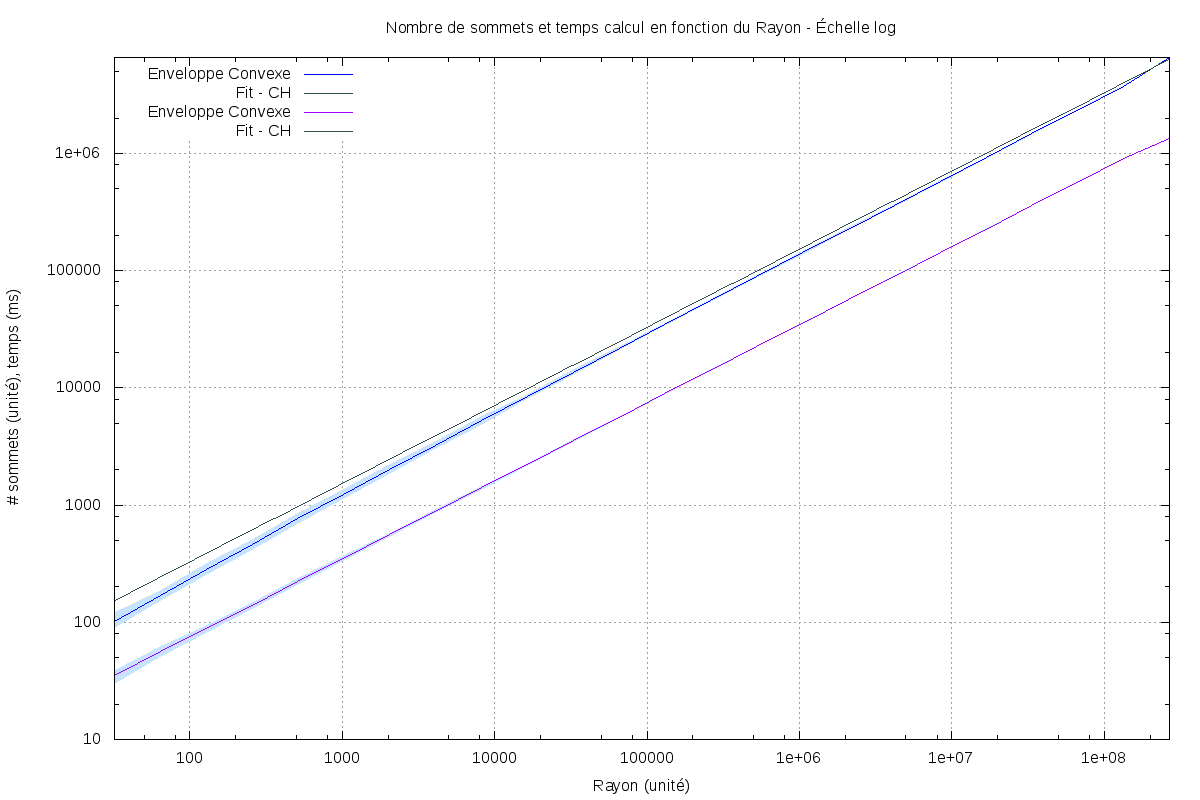
\includegraphics[width=\linewidth]{fig/4-exi/ch/exi-ch-sommet.png}
  \caption{Sommets et bord de l'enveloppe convexe}
\end{figure}

\begin{table}[h!]
  \begin{tabular}{|p{0.09\linewidth}|p{0.13\linewidth}||p{0.2\linewidth}|p{0.13\linewidth}||p{0.2\linewidth}|p{0.13\linewidth}|}
    \hline
    \multicolumn{2}{|c||}{Rayon} & \multicolumn{4}{c|}{Enveloppe convexe} \\  \hline 
    $R=2^k$  &  & \multicolumn{2}{c||}{Nombre de Sommets} &  \multicolumn{2}{c|}{Nombre de points sur le bord} \\ \hline 
    k & R &   & $\# / R^{2/3}$  &   & $\# / R^{2/3}$ \\    
    \hline
    5 & 32 & 35,36 & 3,51 & 102,05 &  10,12\\
    6 & 64 & 55,78 & 3,49 & 170,16 &  10,64\\
    7 & 128 & 87,78 & 3,46 & 283,69 &  11,17\\
    8 & 256 & 139,71 & 3,47 & 465,06 &  11,53\\
    9 & 512 & 222,07 & 3,47 & 761,01 &  11,89\\
    10 & 1024 & 351,72 & 3,46 & 1,24E+03 &  12,21\\
    11 & 2048 & 558,18 & 3,46 & 2,01E+03 &  12,45\\
    12 & 4096 & 883,86 & 3,45 & 3,24E+03 &  12,68\\
    13 & 8192 & 1,40E+003 & 3,45 & 5,25E+03 &  12,92\\
    14 & 16384 & 2,23E+003 & 3,45 & 8,41E+03 &  13,03\\
    15 & 32768 & 3,54E+003 & 3,45 & 1,35E+04 &  13,19\\
    16 & 65536 & 5,62E+003 & 3,46 & 2,16E+04 &  13,28\\
    17 & 131072 & 8,91E+003 & 3,45 & 3,47E+04 &  13,45\\
    18 & 262144 & 1,41E+004 & 3,45 & 5,54E+04 &  13,53\\
    19 & 524288 & 2,25E+004 & 3,45 & 8,87E+04 &  13,64\\
    20 & 1048576 & 3,56E+004 & 3,45 & 1,42E+05 &  13,75\\
    21 & 2097152 & 5,66E+004 & 3,45 & 2,26E+05 &  13,81\\
    22 & 4194304 & 8,98E+004 & 3,45 & 3,61E+05 &  13,88\\
    23 & 8388608 & 1,43E+005 & 3,45 & 5,76E+05 &  13,94\\
    24 & 16777216 & 2,26E+005 & 3,45 & 9,19E+05 &  14,02\\
    25 & 33554432 & 3,59E+005 & 3,45 &  1,46E+06  &  14,07\\
    26 & 67108864 & 5,70E+005 & 3,45 &  2,33E+06  &  14,10\\
    27 & 134217728 & 8,98E+005 & 3,42 &  3,74E+06  &  14,27\\
    28 & 268435456 &  1,35E+06  & 3,24 &  6,62E+06  &  15,90\\
    \hline
  \end{tabular} 
  \caption{Sommet et bord de l'enveloppe convexe}
\end{table}

\begin{figure}[h!]
  \centering
  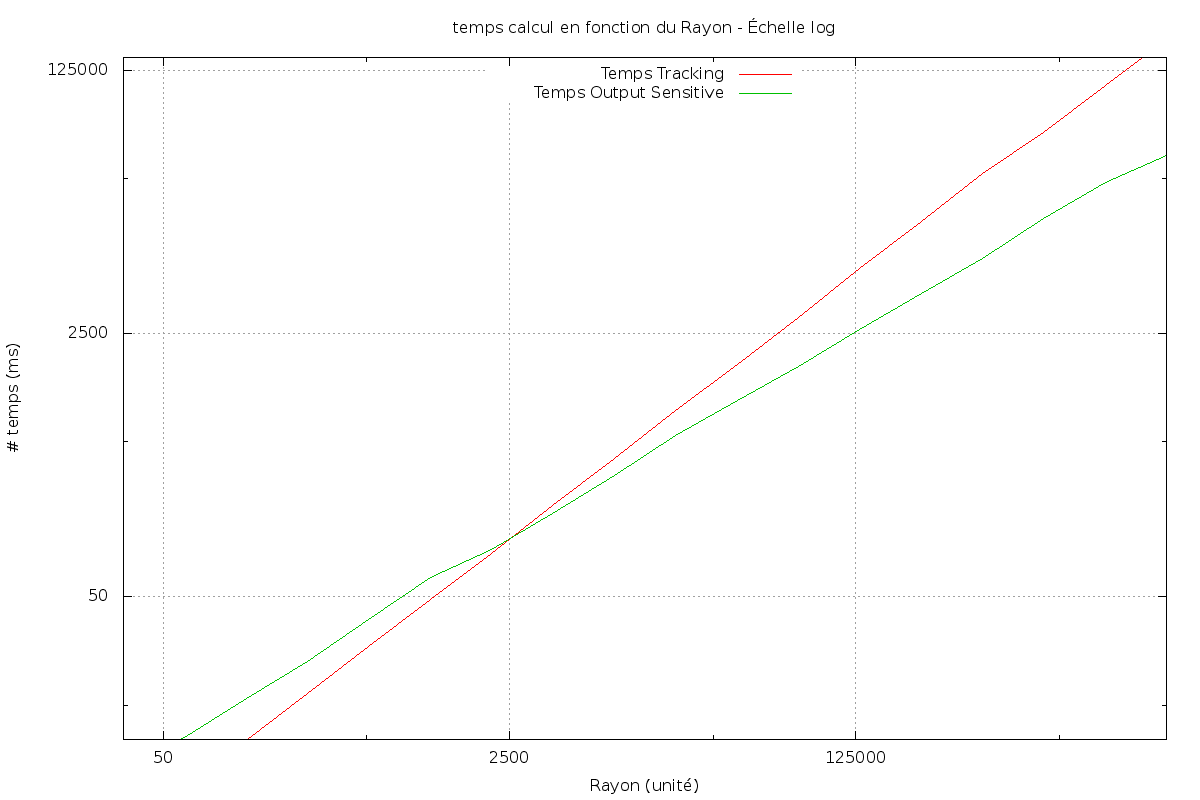
\includegraphics[width=\linewidth]{fig/4-exi/ch/exi-ch-temps.png}
  \caption{Temps de calcul de l'enveloppe convexe}
\end{figure}

\begin{table}[h!]
  \begin{tabular}{|p{0.09\linewidth}|p{0.13\linewidth}||p{0.23\linewidth}|p{0.23\linewidth}|p{0.23\linewidth}|}
    \hline
    \multicolumn{2}{|c||}{Rayon} & \multicolumn{3}{c|}{Temps de calcul (ms) } \\  \hline 
    $R=2^k$  &  &  \multicolumn{3}{c|}{Enveloppe Convexe}  \\ \hline
    k & R & Marche de Grahaam & Har-Peled - Sommets & Har-Peled - Bord \\
    \hline
    5 & 32 & 0,64 & 1,05 &  1,98\\
    6 & 64 & 1,18 & 1,87 &  3,77\\
    7 & 128 & 2,33 & 3,3 &  7,08\\
    8 & 256 & 4,64 & 5,86 &  13,02\\
    9 & 512 & 9,25 & 10,29 &  23,99\\
    10 & 1024 & 32,5 & 17,9 &  43,34\\
    11 & 2048 & 37,03 & 31,13 &  78,05\\
    12 & 4096 & 74,55 & 53,75 &  139,12\\
    13 & 8192 & 149,03 & 92,57 &  247,36\\
    14 & 16384 & 297,79 & 159,44 &  433,88\\
    15 & 32768 & 596,22 & 272,74 &  760,20\\
    16 & 65536 & 1,19E+03 & 466,51 &  1,32E+003\\
    17 & 131072 & 2,37E+03 & 795,09 &  2,30E+003\\
    18 & 262144 & 4,73E+03 &  1,35E+003  &  3,99E+003\\
    19 & 524288 & 9,47E+03 &  2,29E+003  &  6,88E+003\\
    20 & 1048576 & 1,89E+04 &  3,88E+003  &  1,18E+004\\
    21 & 2097152 & 3,79E+04 &  6,58E+003  &  2,02E+004\\
    22 & 4194304 & 7,58E+04 &  1,11E+004  &  3,45E+004\\
    23 & 8388608 & 1,52E+05 &  1,86E+004  &  5,88E+004\\
    24 & 16777216 & 3,03E+05 &  3,13E+004  &  1,00E+005\\
    25 & 33554432 &  &  5,26E+004  &  1,70E+005\\
    26 & 67108864 &  &  8,80E+004  &  2,87E+005\\
    27 & 134217728 &  &  1,46E+005  &  4,82E+005\\
    28 & 268435456 &  &  2,33E+005  &  8,85E+005\\
    \hline
  \end{tabular} 
  \caption{Temps de calcul de l'enveloppe convexe}
\end{table}


Nos résultats obtenus sont conformes à ceux de la publication \cite{HarPeled98}. On remarque que la moyenne asymptotique par rayon de la division du nombre de sommets de l'enveloppe convexe sur le rayon à la puissance 2/3 est 3,45. Des anomalies commencent à apparaitre pour des rayons de la taille de $2^{27} = 134217728$. Il convient de chercher à comprendre d'où elles viennent afin de mieux cerner les possibles limitations de notre algorithme.\\

Le graphique représentant les temps est également intéressant. On observe avec l'echelle logarithmique que la complexité en temps est sous-linéaire pour la méthode de Har-Peled. La méthode devient d'ailleurs plus intéressante en terme de temps de calcul à partir d'un certain rayon : .




